% 89-04(89쪽) — $\seg{AB}=3\sqrt{2}$, $A=105^\circ$, $B=45^\circ$ 인 삼각형 ABC 와 변 BC 위의 점 P(원문 「오른쪽 그림」).
% 스캔 화질이 낮아 TikZ 로 다시 그림. 라벨은 원문 것만 — 네 점 이름, $3\sqrt{2}$, $105^\circ$, $45^\circ$.
% $\seg{CP}/\sin(\angle\pt{CAP})$ 의 최솟값(답)이 읽히지 않게 눈금은 넣지 않는다.
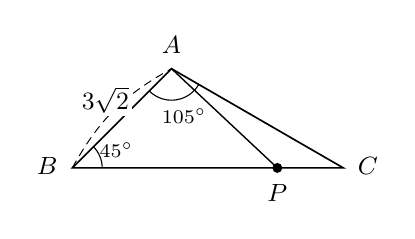
\begin{tikzpicture}[line width=0.6pt]
  \coordinate (A) at (1.26,1.26);
  \coordinate (B) at (0,0);
  \coordinate (C) at (3.442,0);
  \coordinate (P) at (2.604,0);
  \draw (A) -- (B) -- (C) -- cycle;
  \draw[line width=0.5pt] (A) -- (P);
  \fill (P) circle (1.8pt);
  % $105^\circ$ = $\angle\pt{BAC}$
  \draw[line width=0.4pt] (0.977,0.977) arc (225:330:0.40);
  \node[font=\scriptsize] at (1.42,0.66) {$105^\circ$};
  % $45^\circ$ = $\angle\pt{ABC}$
  \draw[line width=0.4pt] (0.38,0) arc (0:45:0.38);
  \node[font=\scriptsize] at (0.56,0.23) {$45^\circ$};
  % 길이 표시의 점선 호
  \draw[densely dashed, line width=0.35pt] (B) to[bend left=16] (A);
  \node[font=\small, fill=white, inner sep=1pt] at (0.42,0.86) {$3\sqrt{2}$};
  \node[font=\small, anchor=south] at (1.26,1.32) {$\pt{A}$};
  \node[font=\small, anchor=east] at (-0.06,0.02) {$\pt{B}$};
  \node[font=\small, anchor=west] at (3.50,0.02) {$\pt{C}$};
  \node[font=\small, anchor=north] at (2.604,-0.08) {$\pt{P}$};
\end{tikzpicture}
